\chapter{Installation}

Before installing ClockAlarm some requirements have to be fulfilled: the
installed Python version should be at least 3.6 and the following packages have
to be installed:

\begin{itemize}
    \item pygame >= 1.9.3
    \item PyQt5 >= 5.8.2 
    \item sip >= 4.19.2
    \item tinydb >= 3.2.2 
\end{itemize}

This can be done with one command: ``\texttt{pip3 install pygame pyqt5 sip
tinydb}''.
The repository can be cloned: ``\texttt{git clone
https://github.com/BFH-BTI7301-project1/ClockAlarm.git}''.
The program can finally be run using: ``\texttt{python3 bin/clockalarm}''.

\begin{figure}[h]
    \centering
    \caption{ClockAlarm main window}
    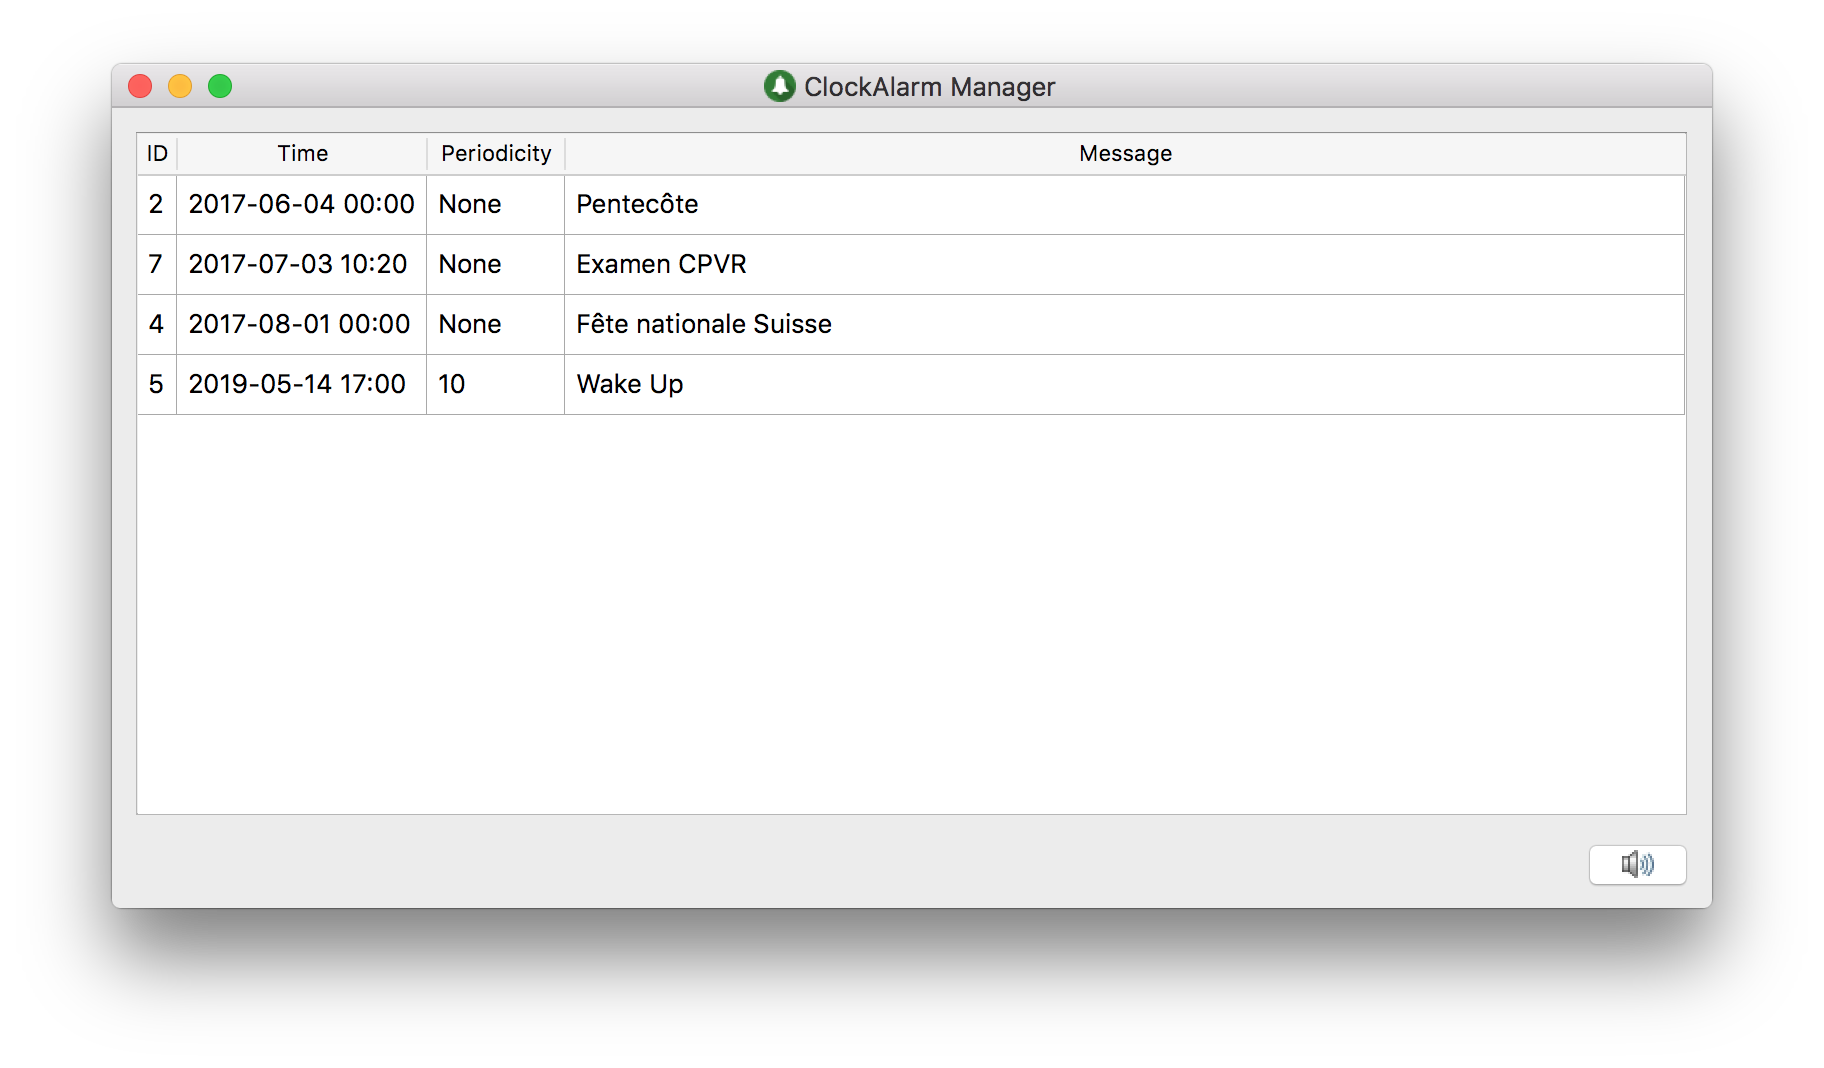
\includegraphics[width=0.9\textwidth]{main_window.png}
\end{figure}

To run the tests these packages have to be installed:

\begin{itemize}
    \item coverage >= 4.4.1
    \item pytest >= 3.0.7
    \item pytest-cov >= 2.5.1
    \item pytest-qt >= 2.1.0
    \item pytest-catchlog >= 1.2.2
    \item coveralls >= 1.1
\end{itemize}

Then the following command should be executed in the project directory:
``\texttt{py.test --cov-report term --cov=. \_clockalarm/\_tests}''. This will
run the tests and output a coverage report in the terminal. To get an html
report, change the argument \texttt{term} to \texttt{html}. The generated html
can be found under \texttt{ClockAlarm/htmlcov/}. Open the \texttt{index.html} to
get the coverage report.

To generate the documentation make sure that Sphinx (>=1.6.1) is installed. Use
``\texttt{make html}'' in the directory \texttt{ClockAlarm/docs/} to generate the
documentation in html format. The output is located under
\texttt{ClockAlarm/docs/\_build/html}. It is possible to change the format, to
see which are available execute only ``\texttt{make}''.
